% Cross-modal retrieval is not only an important task in itself but it is also helpful in evaluating emerging and creative generative models like stable-diffusion and large language models.
\section{Evaluating Cross-modal Generative Models Using Retrieval Task}
\label{sec:gnn_exp_bench}

Multimodal learning has grown rapidly in recent years with pre-trained vision-language models~\cite{CLIP, VILT}. Image-to-text generation, also known as image captioning, has made significant progress in generating captions that are indistinguishable from those written by humans. The task uses an image as input and generates its natural language description. Some of the captioning models, including BLIP~\cite{BLIP}, and GIT~\cite{GIT} are generative unified transformer frameworks that have been trained on multiple tasks involving different modalities, whereas others such as ClipCap~\cite{ClipCap}, MAPL~\cite{MAPL}, and FROZEN~\cite{Frozen} have only been trained on the image captioning task. 

\subsection{Related Work}
Various reference-based, reference-free, and self-retrieval-based methods are used to evaluate and compare the effectiveness of image captioning models in generating valid and descriptive captions for a given image. The majority of these reference-based evaluation metrics, such as BLEU~\cite{bleu}, CIDEr~\cite{CIDEr}, METEOR~\cite{METEOR}, and ROUGE~\cite{ROUGE}, investigate the co-occurrence frequency of n-grams in the predicted caption in comparison to five human-written reference captions, whereas methods like SPICE~\cite{Anderson2016SPICESP} apply a semantic parser to a set of references and compute similarity using the predicted scene graph. Popular embedding-based metrics, such as BERTScore~\cite{BERTScore}, employ contextual embeddings to represent tokens and compute matching using cosine similarity, optionally weighted with inverse document frequency scores. CLIPScore~\cite{CLIPScore}, a popular reference-free evaluation metric, computes the cosine similarity between features extracted from the image and candidate caption using CLIP's feature extractor. The self-retrieval-based evaluation ranks the set of original images using the generated caption as the query to produce a ranked list. It computes the top-k recalls based on the ranked lists, which is the proportion of images within the top-k positions of the ranked lists for each query. The top-k recall is an excellent indicator of how well a model captures distinctiveness in its descriptions. Our proposed text-to-image retrieval task is a combination of reference-based and self-retrieval-based methods, favoring the generation of semantically relevant and unique captions in its evaluations.
\par Text-to-image generation, also known as image generation, has also made significant progress in generating high-quality photo-realistic images from a given text prompt. These models are mainly divided into four groups, namely normalizing flows \cite{JimenezRezende2015VariationalIW}, VAE \cite{Kingma2013AutoEncodingVB}, GAN \cite{Goodfellow2014GenerativeAN} and diffusion models \cite{stable-diffusion, IMAGEN, DALLE2}. The task uses an input text prompt to generate a semantically similar image from the latent space. Some of the recent models are diffusion-based models, which include DALL-E\cite{DALLE}, DALL-E 2\cite{DALLE2}, minDALL-E \cite{minDALL-E}, Stable Diffusion \cite{stable-diffusion}, GLIDE \cite{GLIDE}, Make-A-Scene \cite{MakeAScene}, and IMAGEN \cite{IMAGEN}. We require an empirical measure to evaluate and compare these implicit image-generative models. The most common metrics used are Inception Score (IS), Fréchet Inception Distance (FID), and Fréchet CLIP Distance (FCD) \cite{Betzalel2022ASO}. The IS uses an Inception-v3 Network pre-trained on ImageNet and calculates a statistic of the network’s outputs when applied to generated images. FID computes Fréchet Distance between two multivariate Gaussians, fitted to the features extracted by the Inception network at pool3 layer for real and generated data. As these metrics are based on features and scores computed using a pre-trained network on ImageNet \cite{ImageNet} dataset with a particular image size, it is unclear how well they transfer to other image types and sizes. In contrast to the heuristic-based metric, our proposed retrieval task models the user behavior and judgment of relevant items. It also uses the pre-trained transformer-based models trained on large-scale data to provide robustness to different data types and sizes.

\subsection{CMR Framework for Evaluation}
In this work, we investigate whether the heuristics-based metrics such as CLIPScore, BLEU-4, FID, etc. used for evaluating cross-modal generative models are consistent with systematic metrics for ranked retrieval evaluation such as nDCG\textquotesingle@K~\cite{Sakai2008OnIR} and RBP\textquotesingle@K~\cite{Moffat2008RankbiasedPF}. For this purpose, we propose a novel unified cross-modal retrieval (CMR) framework that computes a ranking of results for a given query by making use of a cross-modal generative model. The CMR framework, as depicted in Figure \ref{fig:framework}, consists of a set of human-written captions and real-world images as ground truth reference queries, a retrieval system, a set of generated items (captions and images) as new retrieval set, a generative model for evaluation, an input retrieval set of images and textual prompt, and a set of evaluation metrics (nDCG\textquotesingle@K and RBP\textquotesingle@K).


\begin{figure*}[htbp]
\centering
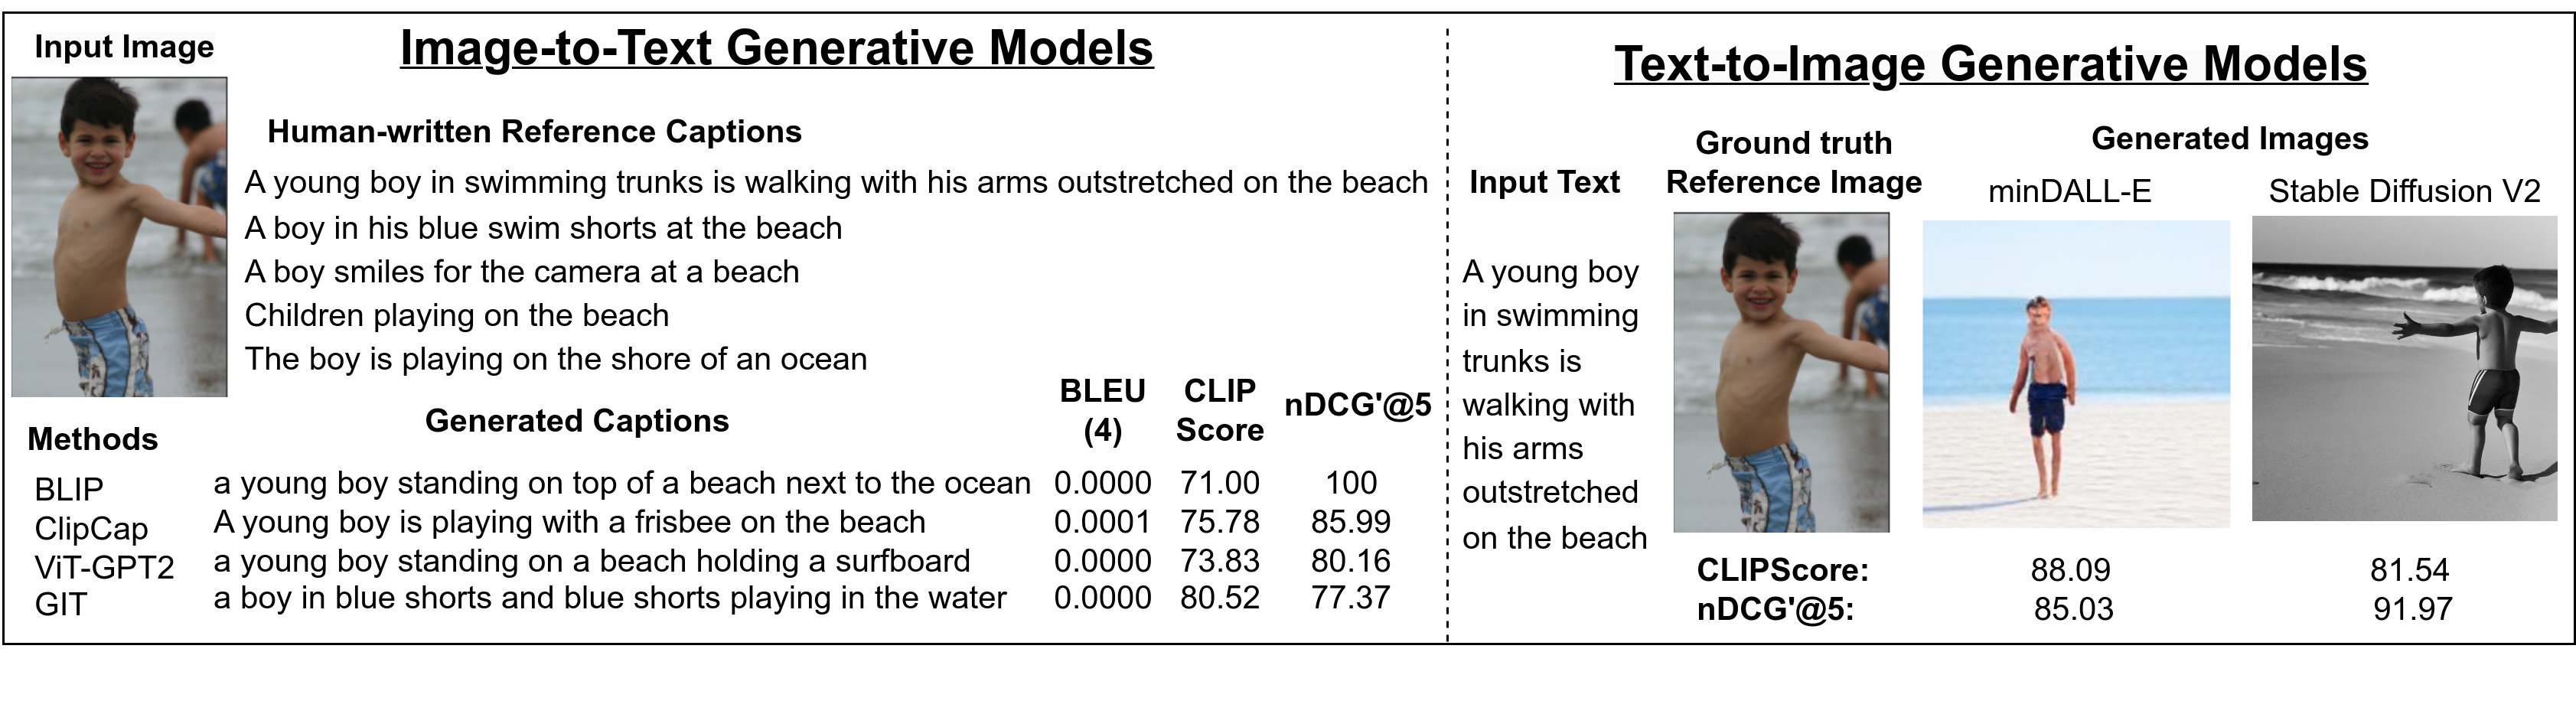
\includegraphics[width=\textwidth]{Figures/demo_two.png}
\vspace*{-8mm}
\caption{Example showing shortcomings of well-known n-gram matching and embedding-based metrics}
\label{fig:demo}
\end{figure*}

\begin{figure*}[htbp]
\centering
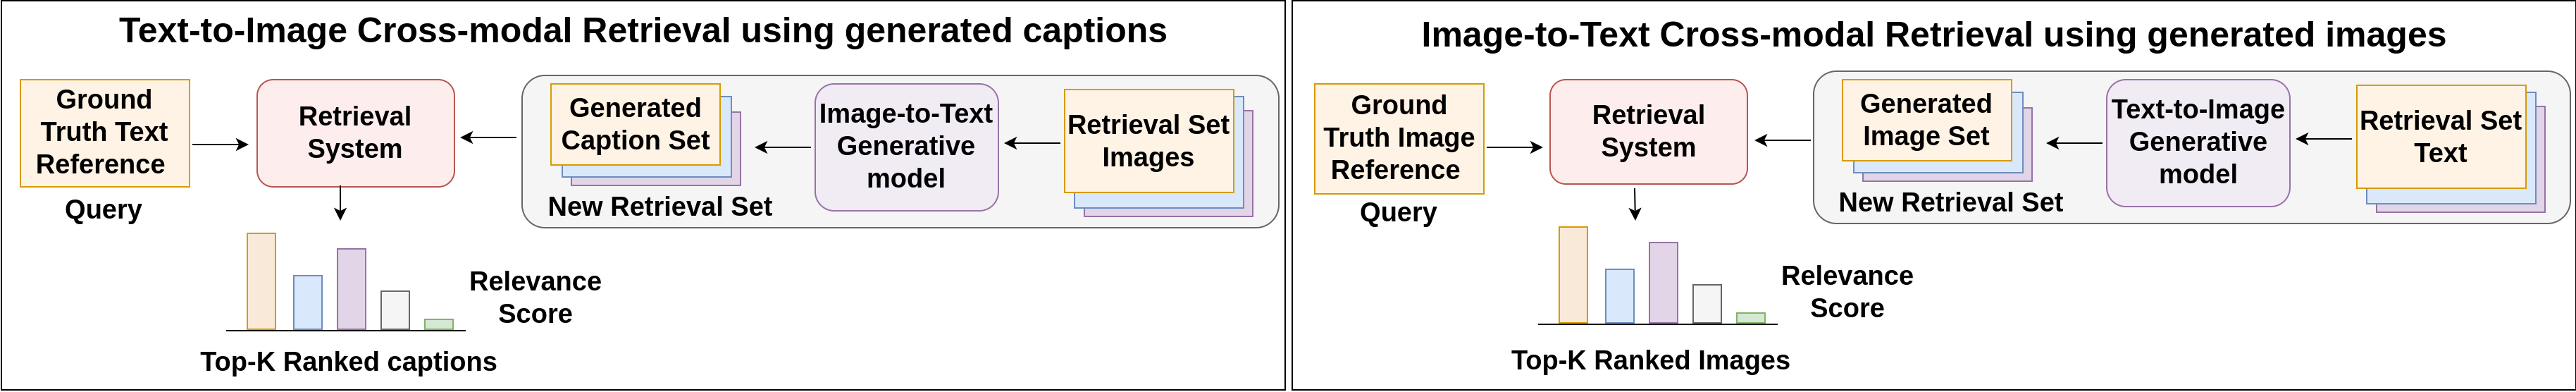
\includegraphics[width=\textwidth]{Figures/both.png}
\vspace*{-8mm}
\caption{Cross-modal Retrieval Framework to Evaluate Generative Models.}
\label{fig:framework}
\end{figure*}

\noindent\textbf{Evaluation of Image Captioning Models:}
The evaluation of the image captioning model can be framed as a text-to-image retrieval task as shown on the left side of Figure \ref{fig:framework}. This procedure encourages the image captioning model to generate a semantically similar caption for the input image that not only describes the image scene but is also unique in its description. A semantically similar caption will be able to rank the human-annotated relevant images at the top when the ground truth reference caption is used as the query. First, we feed the set of input images \textit{X}, one by one to the caption generation model, say BLIP, to generate a single caption candidate $y$. The generated candidate caption set \textit{Y} forms the new retrieval set used as an intermediary for the cross-modal retrieval task. Then we perform the text-to-image retrieval task, using the corresponding ground truth reference caption $y_x$ as the query to rank the generated caption set \textit{Y} and its mapped image set \textit{X} using cosine similarity score. Finally, we evaluate the ranking of the top-k images based on the available human-annotated graded relevance score using nDCG\textquotesingle@K and RBP\textquotesingle@K metrics. The higher the ranking score, the better the image captioning model.

\noindent\textbf{Evaluation of Image Generation Models:}
Figure \ref{fig:framework} on the right shows the reverse procedure of the evaluation of the image generative model, framed as an image-to-text retrieval task. This procedure encourages the image generation model to generate a semantically similar image that is not only representative of the input textual prompt but also photo-realistic and unique. A semantically similar image will be able to rank the human-annotated relevant textual prompts at the top when the ground truth real image is used as a query. First, we feed the set of input textual prompts \textit{Y}, one by one to the text-conditioned image synthesis model, say minDALL-E, to generate a single image candidate $x$. The generated candidate image set \textit{X} forms the new retrieval set used as an intermediary for the cross-modal retrieval task. Then we perform the image-to-text retrieval task, using the corresponding ground truth reference image $x_y$ as the query to rank the generated image set \textit{X} and its mapped textual prompt set \textit{Y} using cosine similarity score. Finally, we evaluate the ranking of the top-k textual prompt based on the available human-annotated graded relevance score using nDCG\textquotesingle@K and RBP\textquotesingle@K metrics. The higher the ranking score, the better the image generation model.

\subsection{Experimental Results}
We conduct an experimental evaluation using \textit{ECCV Caption}~\cite{ECCV} and \textit{Flickr8k-EXPERTS} benchmarks, which contain graded (albeit shallow) relevance assessments. The two datasets are extended subsets of the COCO Caption \cite{Lin2014MicrosoftCC} and Flickr-8K datasets \cite{flickr8k}, respectively. ECCV Caption includes 1,332 query images and 1,261 query captions, while Flickr8k-EXPERTS includes 1,000 images and 977 captions. 
% The dataset contains a rating score of image-caption pairs given by human experts on a scale of 0 to 3, with 0 indicating that the caption does not describe the image at all, 1 indicating that the caption describes minor aspects of the image but does not describe the image, 2 indicating that the caption almost describes the image with minor errors, and 3 indicating that the caption describes the image.

% Cross-modal Retrieval
We address these two research questions in our experiments:\\
\textbf{RQ1:} What is the ranking effectiveness of generative models in CMR task? \\
\textbf{RQ2:} Are heuristics-driven metrics used in generative model evaluation consistent with results from user-behavior-driven metrics such as \textit{nDCG\textquotesingle@K} and \textit{RBP\textquotesingle@K}? 

\begin{table*}[htbp]
\centering
\caption{Evaluation of Image-to-Text Generative Model on ECCV Caption and Flickr8k-EXPERTS Dataset. Bold fonts and underline indicate the best performer and the second-best performer, respectively. Results marked $\dagger$ are statistically significant (i.e., two-sided t-test with \textit{p} $\leq$  0.05) over the second-best method.}
\label{tab:eccv-caption}
\resizebox{0.7\textwidth}{!}{
\begin{tabular}{@{}cc ccc c@{}}
\toprule 
Dataset      & Method & nDCG\textquotesingle@10 & RBP\textquotesingle@10 & BLEU-4 $\uparrow$ & CLIPScore $\uparrow$ \\ \midrule
ECCV Caption & ClipCap & 87.96 & 1.87  & 33.3  & 77.6 \\
ECCV Caption & ViT-GPT2 & 88.4 &  \underline{1.88} &  \underline{39.2} & 75.4   \\
ECCV Caption & GIT & \underline{88.74} &  \underline{1.88} & 37.8 & \textbf{77.9}$\dagger$ \\
ECCV Caption & BLIP & \textbf{89.15}$\dagger$ & \textbf{1.89}$\dagger$ & \textbf{41.7}$\dagger$ & \underline{77.8} \\
\midrule
Flickr8k-EXPERTS & ClipCap & 70.23 & 0.85  & 18.69 & 77.55 \\
Flickr8k-EXPERTS & ViT-GPT2 & 69.32 &  0.83 & \underline{25.68} &\textbf{78.53}$\dagger$  \\
Flickr8k-EXPERTS & GIT & \underline{71.08} & \underline{0.87}  & 17.21 & 71.47 \\
Flickr8k-EXPERTS & BLIP & \textbf{69.83} &  \textbf{0.88}$\dagger$ & \textbf{29.14}$\dagger$ &	\underline{77.81} \\
\bottomrule
\end{tabular}
}
\end{table*}

\begin{table*}[htbp]
\centering
\caption{Evaluation of Text-to-Image Generative Model on ECCV Caption and Flickr8k-EXPERTS Dataset. Bold fonts indicate the best performer method. Results marked $\dagger$ are statistically significant (i.e., two-sided t-test with \textit{p} $\leq$  0.05) over the second-best performer.}
\label{tab:eccv-image}
\resizebox{0.7\textwidth}{!}{
\begin{tabular}{@{}cc ccc c@{}}
\toprule 
Dataset & Method & nDCG\textquotesingle@10 & RBP\textquotesingle@10 & FID $\downarrow$ & CLIPScore $\uparrow$\\ 
\midrule
ECCV Caption & MinDALL-E &	77.85 & 2.16 & 50.61 & 78.68\\
ECCV Caption & SDV2 &	\textbf{81.02}$\dagger$ & \textbf{2.28}$\dagger$ & \textbf{18.31} & \textbf{83.07}$\dagger$ \\
\midrule
Flickr8k-EXPERTS & MinDALL-E & 75.02 & 0.90 & 99.99 & 79.66 \\
Flickr8k-EXPERTS & SDV2 & \textbf{77.03}$\dagger$ & \textbf{0.95}$\dagger$ & \textbf{63.38} & \textbf{85.88}$\dagger$\\
\bottomrule
\end{tabular}
}
\end{table*}


\par In Table \ref{tab:eccv-caption}, nDCG\textquotesingle@K and RBP\textquotesingle@K compare the performance of image-captioning models on ECCV Caption and Flickr8k-EXPERTS. The BLIP model gets the highest nDCG\textquotesingle@K and RBP\textquotesingle@K scores in comparison to other models for both datasets. The same model also outperforms others in heuristics-driven metrics as well. This suggests that BLIP captions are not only semantically more similar to the ground truth reference captions but also can better rank images in the retrieval task. This is also evident from the example in Figure \ref{fig:demo}. With respect to RQ2, we notice that CLIPScore is inconsistent with ranking metrics for different models -- the GIT and ViT-GPT2 models get the highest CLIPScore on the ECCV Caption and Flickr8-EXPERTS respectively. It is also interesting to note that there is a bigger spread of CLIPScore values for different models on the Flickr8k-EXPERTS dataset, than nDCG\textquotesingle@K and RBP\textquotesingle@K scores. The images generated by the Stable Diffusion V2 (SDV2) and minDALL-E models are compared for their ranking effectiveness in Table \ref{tab:eccv-image}. The results suggest that the SDV2 model generates a more similar image for a given text input that is also distinct from the set of generated images in order to rank textual prompts more effectively in the retrieval task for both datasets. Also, there is a huge gap in the FID Score for the two models, which is not the case with nDCG\textquotesingle@K and RBP\textquotesingle@K scores.

\subsection{Conclusion}
We explored whether heuristics-based metrics used for evaluating image-to-text and text-to-image generative models are consistent with models such as nDCG\textquotesingle@K and RBP\textquotesingle@K that are based on robust user behavior models. We presented a novel unified cross-modal retrieval framework that uses generative models for the retrieval task and used it in our comparison of metrics. Empirically we showed the interpretability challenge with the heuristics metrics and showed that nDCG\textquotesingle@K and RBP\textquotesingle@K are more suitable in terms of their interpretability and usability. Further investigation is needed to use the nDCG\textquotesingle@K and RBP\textquotesingle@K metrics to tune the underlying models, and also to develop better evaluation benchmarks with graded judgments further deep in rankings. 